\documentclass[12pt,a4paper]{article}
\usepackage[left=25mm,right=15mm,top=15mm,bottom=15mm]{geometry}
\usepackage[utf8x]{inputenc}
\usepackage[L7x]{fontenc}
\usepackage[lithuanian]{babel}
\usepackage{url}
\usepackage{float}
\usepackage{graphicx}
\renewcommand{\baselinestretch}{1.5}
\graphicspath{ {img/} }

\begin{document}
\begin{titlepage}
  
  \begin{center}
    \textsc{\LARGE Vilniaus Gedimino Technikos universitetas}\\[2mm]
    \textsc{\Large Elektroninių sistemų katedra}\\[70mm]
    \textsc{\Large Atviro programinė įranga}\\[10mm]
    \textsc{\normalsize Kursinis darbas}\\[40mm]
    \begin{minipage}{1\textwidth}
      \begin{flushright}
        \emph{Darbą atliko:} Maksim Norkin, AKSfm-15\\
        \emph{Darbą tikrino:} Doc. Raimondas Pomarnacki\\
      \end{flushright}
    \end{minipage}
    \vfill
    {\large Vilnius \\ \the\year}
  \end{center}
\end{titlepage}
\tableofcontents
\newpage

\section{Įvadas. Užduoties analizė}

Objekto padėties nustatymas turi dvi plačias pritaikymo sritis: inercinė navigacinė ir žmogaus judesio sekimo sistema \cite{schlomer2008gesture};

Objekto pozicijos nustatymas, panaudojus inercinius jutiklius remiasi prielaida, jog objektas lieka ramybės būsenoje tol, kol jį nepaveikia išorinė jėga. Tokia jėga suteikia objektui pagreitį. Jeigu rasta pagreitį galima išmatuoti ir suintegruoti, pagreičio ir pozicijos kitimas gali būti išmatuoti. Reikia nepamiršti, kad tokiu atveju matavimą sudarys dvi komponentės -- pagreitis dėl gravitacijos ir išorinės veikiančios jėgos pagreitis. Norint pašalinti gravitacijos komponentę iš pagreičio matavimo, reikia žinoti kokiu kampu akcelerometras yra vertikalės atžvilgiu.
Tokio kampo matavimui, reikalingas kitas jutiklis, kuris vadinasi giroskopas. Jis matuoja kampo greitį, kurį matematiškai integruojant, galima rasti kampo greičio pokytį nuo pradinio, žinomo kampo \cite{sukkarieh2000low}.

Akcelerometras suteikia pagreičio matavimą norimam objektui. Dažniausiai tokie matavimai yra užrašomi $x$, judėjimą tiesiai, $y$, šonu ir $z$ vertikaliai. Giroskopas suteikia matavimus, kurie dengia nurodytas ašis ir yra užrašomi $\theta$, sūkiui, $\beta$ polinkiui ir $\gamma$ vingiavimui, kaip pavaizduota \ref{tikz:axis_of_the_system} pavyzdyje. Tokių inercinių įverčių naudojimas turi pagrindinį privalumą -- stebimo objekto polinkis ir pagreitis gali būti vertinami bet kokioje navigacijoje.  

\begin{figure}[H]
    \centering
    \caption{Objekto pozicijos pagreičio pokyčio ašys, $x$, $y$ ir $z$. Sūkio matmenys apie ašis $\theta$, $\beta$ ir $\gamma$.}
    \label{tikz:axis_of_the_system}
    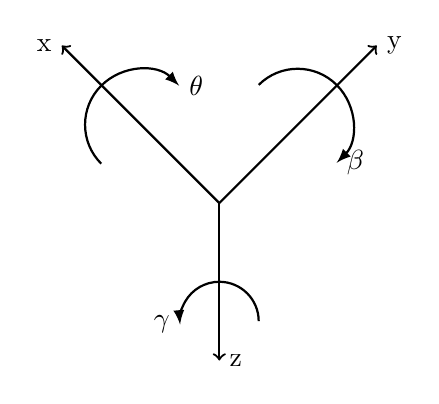
\begin{tikzpicture}
        % axis
        \draw[thick, black, ->] (0,0) -- ( 2, 2) node [right] {y};
        \draw[thick, black, ->] (0,0) -- (-2, 2) node [left] {x}; 
        \draw[thick, black, ->] (0,0) -- ( 0,-2) node [right] {z};
        % arc
        \draw[thick, -latex] ( 0.5,  1.5) arc (135:-45:0.70) node [right] {$\beta$}; 
        \draw[thick, -latex] (-1.5,  0.5) arc (225:45:0.70) node [right] {$\theta$};
        \draw[thick, -latex] ( 0.5, -1.5) arc (0:185:0.5) node [left] {$\gamma$};
    \end{tikzpicture}
\end{figure}

Inercinės navigacijos sistemos yra naudojamos labai plačiai lėktuvuose, raketose, kosmoso laivuose, povandeniniuose ir vandens laivuose \cite{woodman2007introduction}. Progresas gaminant MEMS įrenginius, sudarė galimybes kurti mažas ir lengvas navigacines sistemas. Tokie privalumai leidžia praplatinti įrenginių panaudojimo galimybes ir šiuo metu įtraukia tokias sritis kaip žmogaus ir gyvūnų judesio sekimą.

Tačiau reikia nepamiršti ir apie klaidas, kurias sukelia nuolatinė dedamoji, santykio įverčiai ir nelinijines sistemos įtakos jutiklio verčių nuskaitymo metu. Tokios klaidos yra pagrindinė priežastis atsirasti netikslumams navigacinėje sistemoje per laiko vienetą. Netikslumai sąlygoja akselerometro įverčius, kuriuos tampa labai sunku atskirti tarp gravitacinio lauko ir objekto judėjimo, ko pasekoje objekto pozicijos matavimas toliau yra dar netikslesnis. Kadangi inerciniai jutikliai yra tokio tipo, kuriems yra labai svarbi tiksli prieš tai buvusi pozicija, bet kokia klaida skaičiuojant prieš tai buvusia pozicija, įtakoja ir dabartinės pozicijos skaičiavimą. Tokiu būdu, su laiku navigacinė sistema tampa visiškai netiksli ir praranda visą savo vertę.

\section{Analogiškos paskirties programinės įrangos apžvalga}

Analogiškos programinės įrangos analizė suteikia galimybę detaliau įsivertinti rinkos situaciją ir surasti sprendimą, kuris gali tapti baze kuriamai programinei įrangai.
Kaip alternatyva yra bibliotekų panaudojimas.
Jeigu rastos programinės įrangos licenciją yra nesuderinama su norima naudoti licencija -- galima peržiūrėti naudojamų bibliotekų licencijas, ir jeigu bibliotekų licencijos yra suderinamos su norima naudoti licencija -- panaudoti būtent tas bibliotekas, taip palengvinant visą darbą.

\subsection{Analogiška programinė įranga}

Paprasta programa, kuri yra labai gerai pritaikoma esamai platformai yra \cite{MPU9243:online}. Programinė įranga yra licencijuojama pagal \textit{Beerware} licenciją. Šita licencija leidžia naudoti išeities kodą arba pačią programinę įrangą laisvai, bet kokias tikslais.

\begin{verbatim}
 * MPU9250 Basic Example Code
 * by: Kris Winer
 * date: April 1, 2014
 * license: Beerware - Use this code however you'd like. If you
 * find it useful you can buy me a beer some time.
\end{verbatim}

Pats programinis kodas yra parašytas labai netvarkingai ir yra požymių, kad šis programinis kodas buvo panaudotas iš kito projekto arba kitos įrangos iteracijos, kadangi pačiam projekte yra bibliotekų, kurie neturi visiškai jokios naudojamos srities šiame sprendime. Kaip pavyzdys gali būti LCD ekranas, kurio biblioteka yra įkeliama, tačiau niekur nepanaudota.

Kaip labai panašų sprendimą, kuris mūsų platformai nėra tinkamas, yra \cite{MPU6036:online}. Kontrolinis kodas labai panašus į \textit{MPU 9250} atvejį, skiriasi tik pačio bendravimo su senesniu jutikliu \textit{MPU 6036} programinis kodas. Į šią kategoriją taip pat papuola ir \cite{MPU9152:online}, šiuo atveju jutiklis yra \textit{MPU 9152}

Panaudota licencija yra suderinama su BSD licencija, todėl rastas programinis sprendimas galimas panaudoti ir esamai sistemai.

Reikia paminėti, jog panaudojamas programinis kodas parašytas labai chaotiškai, ir kadangi licencijos reikalavimai neriboja darbo su programine įranga, pats sprendimas yra perrašytas su geresniu pateikimu.

\section{Programinės įrangos kūrimas}

Programinės įrangos kūrimas pirmiausiai pradedamas nuo užduoties analizės.
Užduotis yra sukurti programinę įranga, kuri gali dirbti su \textit{STM32F411} platforma ir bendrauti su \textit{MPU 9250} jutikliu.

\begin{figure}[H]
    \centering
    \includegraphics[width=300px]{img/naudojama-platforma.jpg}
    \caption{Naudojama STM32 platforma.}
    \label{fig:web-idea}
\end{figure}

ARM šeimos naudojama platforma suteikia pakankamai galingus įrankius darbo su sistema. Pats paprasčiausias ir priimtiniausias įrankis jokios patirties įterptinėse sistemose neturinčiam programuotojui yra tiesiogiai tinklapyje veikiantis redaktorius, kuris sugeba pasirūpinti reikiamomis bibliotekomis, bei sukompiliuoti visą reikiamą kodą į vieną binarinę bylą, kurią galima tiesiog perkelti į USB sąsaja prijungta plokšte. \textit{STM32F411} platformoje įmontuotas programuotojas automatiškai perrašo procesoriaus vykdomą programinį kodą ir paleidžia programą.

\begin{figure}[H]
    \centering
    \includegraphics[width=300px]{img/web-idea.png}
    \caption{Per paprastą tinklapį pasiekiama įterptinės sistemos programinės įrangos vystymo sąsaja \cite{mbedC9:online}.}
    \label{fig:web-idea}
\end{figure}

Tačiau toks programinės įrangos vystymas gali būti labai lėtas ir sugeneruoti labai daug parsiuntimo bylų skaičių. 
Dėl šios priežasties perkeliam visą programinės įrangos bibliotekas ir kompiliavimą į lokalią mašiną.
Ta pati internetinė platforma leidžia eksportuoti esamą projektą į GNU Toolchain aplinkos projektą, kartu paruošia ir tvarkingą \textit{Makefile}, kurį pačiam rašyti yra labai problematišką.

Pats kompiliavimas vykdomas labai paprastai dėl gražaus \textit{Makefile}, kuris yra sugeneruotos ankščiau aprašytos platformos. Viso labo ką reikia padaryti, tai paleisti \textit{make} komandą terminale ir bus pateikiama bin bylą, kurią toliau reikia įrašyti į įterptinę įrangą. 

Rašymas į įterptinę sistemą vykdomas taip pat konsolės pagalba, naudojant \textit{stlink} programinį paketą. Rašymo komanda \textit{st-flash} pradžioje priima operacijos komanda, kuri rašymo atveju yra \textit{write}, toliau seka objekto byla, kuria norime įrašyti į įterptinę sistemą, \textit{main.bin}, bei galutinis argumentas yra pradžios adresas, \textit{0x8000000}. Visa komanda ir galimas programos išvedimo rezultatas yra pateikiamas \ref{fig:st-link-write} pavyzdyje.

\begin{figure}[H]
    \centering
    \includegraphics[width=500px]{img/st-link-write.png}
    \caption{Programinio patekto \textit{stlink} bin bylos rašymas į įterptinę sistemą.}
    \label{fig:st-link-write}
\end{figure}

Pagaminta programinė įranga yra pateikiama atvirai prieigai, pritaikant BSD licenciją.

\begin{quote}
    https://github.com/dummas/upgraded-giggle
\end{quote}


\section{Programinės įrangos licencijavimas}

\subsection{Apžvalga}

Fundamentinis atviro kodo licencijavimo tikslas yra užkirsti kelią piktybiškai išnaudoti darbą \cite{Laurent:2004:UOS:1096111}.
Tradiciškai, jeigu kūrėjas nori, kad jo darbas pasiektų bent kažkokią publiką ir galiausiai turėti kažkokį pragyvenimo šaltinį iš šio kūrinio, kūrėjas turi atiduoti arba visas, arba dalį autorinių teisių tiems veikėjams, kurie sugeba paskirstyti ir, žinoma, išnaudoti tą darbą.

Kadangi tokie veikėjai, iš prigimties, nemato atlikto darbo, kaip \textit{darbo}, o daugiau žiūri kaip į srautą pinigų, kurį generuoja to darbo išnaudojimas, jie pavydi savo išskirtinėmis teisėmis į produktą.
Jie taip pat nėra linkę dalintis bet kokiu gaunamu pelnu su kitais.
Kadangi potencialūs literatūros ar muzikos darbo naudotojai bus limituoti tik esančia kūrinio pagaminimo kaina, kuri yra nustatoma išskirtinai žmogumi ar veikėju, kuris kontroliuoja teisėmis į prekės paskirstymą -- rinka vers mažinti kainą, norint padidinti pelną.
Kadangi skirtumas kainų tarp jos pagaminimo ir jos pardavimo dažniausiai yra maži -- kuo didesnis pardavimų skaičius su mažesne kaina generuos daugiau pelno leidėjui.

Tokio proceso rezultate, leidėjai labai agresyviai gina autorines teises nuo nelicencijuotų kūrinių paskirstymų ar nuo kitų darbų, kurie paremti apgintu kūriniu.
Meno darbo atveju, problema yra nelicencijuotas originalaus kūrinio paskirstymas. 
Nelicencijuota išvestis dažniausiai suveikia, ir dėl to yra skelbiami ieškiniai kitų asmenų kryptimi, meno kūrinio vertė yra paremta ant originalios išraiškos formos, t.y. kūrinys nėra dinaminis.

Palyginus, programinė įranga yra kartu funkcinė ir dinaminė.
Kiekviena programa susideda iš kodo, kuris kartu yra funkcinis, darbo prasme, ir dinaminis iš konteksto pusės -- programa gali dirbti su plačiu rėžiu užduočių ir aplinkų.
Tokiu rezultatu, sukurta programa vaizduoja du tipus vertės.
Pirma vertė yra formali paskirtis, kaip duomenų bazės sistema ar kita sritis.
Antra vertė yra išeities kodas, kuris potencialiai gali būti panaudotas atlikti kitos paskirties funkcijas.

Kuomet naudotojas nusiperka dalį programinio paketo, kaip pavyzdžiui, \textit{Microsoft Excel}, be fizinės programinės įrangos kopijos ir naudotojo vadovo, jis gauna teisę naudotis programine įranga pagal tiesioginę jo paskirtį -- šiuo atveju kaip skaičiuokles programa. 
Kai tik naudotojas atidaro plastikinę pakuotę, jis automatiškai apribojamas ``shrinkwrap'' licencija, kuri nusako, kad gautą kūrinį negalima kopijuoti, jo pagrindu kurti naują produktą, ir negali suteikti kitoms šalims teisę atlikti tokius veiksmus.
Tokios licencijos pašalinimas yra atviro kodo licencijavimo pagrindas.

Palyginamas atviro kodo licencijuotos programinės įrangos naudotojas yra visiškai kitoje situacijoje.
Jis gali laisvai platinti gautą kopiją (už pinigus arba ne) dėka atviro paskirstymo principo.
Jis gali laisvai ir atvirai keisti gautą darbą ir skirstyti tą pakeistą darbą (vėlgi, už pinigus arba ne) dėka atvirumo keitimams principo.
Vienintelė svarbi darbe su šia teise riba yra platinamo sprendimo, modifikuoto ar ne, licencijavimas turi būti tęstinas su pagrindu panaudoto programinio paketo atvira licencija.

Pavyzdžiui, atviro kodo licencija gali reikalauti modifikuoto darbo paskirstymą su tokiomis pačiomis teisėmis, kaip ir pradinis darbas.
Tai reiškia, kad žmonės, kurie gavo licencijuoto darbo kopiją, ją pakeitė ir pradėjo skirstyti -- jie turi suteikti galimybę kitoms šalims prieiti prie pakeisto sprendimo tokia pačia, arba panašia tvarka, kaip ir pirminiais programinės įrangos variantas.
Toks principas yra vadinamas kartos limitavimas.
Toks limitavimas, priklausomai nuo pradinės licencijos, gali sustabdyti programinį paketą išeiti į uždarą kodą ir verčia atviro kodo naudotojus ir pagalbininkus, teikti sprendimus, kurie yra vertingi atviro kodo bendruomenei.

Atviras kodas skiriasi nuo tradicinio autorinių teisių gynimo licencijavimo, jis leidžia atvirai skleisti ir modifikuoti viską savo poreikiams, antro tipo limitavimo pašalinimas turbūt yra svarbiausias.
Teisės reikalavimas, kad autorinių teisių savininkai kartu suteikia naudotojų keičiamą kodą sprendimams, kuriuos jie gali skleisti ir reikalaujant, kad jie leistų nagrinėjamo darbo vystymą ir skirstymą, atviro kodo licencijavimas suteikia tris svarbius pranašumus prieš tradicinius uždaro kodo komercinius licencijavimo modelius.

Pirmas ir svarbiausias pranašumas yra inovacija.
Šiuo metu jau yra gerai pateikta, kad programinės įrangos vystymo specialistai yra linkę prisidėti prie atviros programinės įrangos projektų, be jokio papildomo atlygio, išskyrus padaryti naudojamą programinį įrankį naudingesnį.
Atviras kodas veikia.
Kuo daugiau programuotojų gali prisidėti prie darbo -- tuo daugiau vertės turės tas programinis paketas.

Antras pranašumas yra patikimumas. 
Daug programuotojų reiškia daug žmonių gali atlikti derinimo darbus.
Ir toks privalumas nėra išreiškiamas skaičiais.
Žinantis naudotojas, kuris atrado klaidą pats savo akimis arba tiesiogiai rankomis yra pajutęs programos limitavimą, gali žymiai geriau surasti klaidą programoje ir ją ištaisyti, negu bet koks darbuotojas, kurio pareigos yra palaikyti programinį paketą.
Toks naudotojas turi žymiai daugiau paskatos pataisyti tokią klaidą duotam programinės įrangos dalyje, jeigu programinės įrangos skirstytojas, kurio prioritetus, kada spręsti tokias klaidas, valdo ir pačio finansiniai ir organizaciniai apribojimai.

Trečias privalumas yra ilgas gyvavimo laikotarpis. Kuomet komerciškai licencijuojamas programinis paketas išeina iš palaikymo, nėra visiškai jokio būdo taisyti tos programinės įrangos klaidų arba dėti naujas savybes.
Toks programinis paketas prieina prie evoliucinio galo.
Palyginimui, atviro programinio kodo projektas gali būti sustabdytas vystymui kažkuriam laikotarpiui, tačiau jis gali būti atgaivintas, pritaikytas arba perrašytas naudotojo arba naudotojų grupės, kurie randa pritaikymą tai programinei įrangai -- ir tas pritaikymas gali būti visiškai skirtingas, negu pradžioje buvo numatyta.

\subsection{MIT, BSD}

MIT ir BSD licencijos, yra dvi pačios seniausios atviro kodo licencijos.
Dėl to, kad šios dvi licencijos yra labai paprastos ir iliustruoja pačius atviro kodo licencijos principus, jie bus aptarti pirmiausiai.
MIT (ar X), BSD ir Apache licencijos yra klasikinės atviro kodo licencijos ir yra panaudotos daugelyje atviro kodo projektuose.
Turbūt daugiausia žinomas yra BSDNet ir FreeBSD Unix šeimos operacinės sistemos ir Apache HTTP serveris.

Šios licencijos, leidžia naudoti programinės įrangos išeities kodą privačiame kode ir nereikalauja publikuoti atliktų pakeitimų.
Kodas, sukurtas naudojant šitas licencijas, gali būti uždaras ir vystymas gali būti vykdomas taikant kitą licenciją, kuri nėra pripažįstama atviro kodo bendruomenės.
Dėl tos pačios priežasties, šitos licencijos yra labai lanksčios ir dera su beveik kiekviena iš atviro kodo licencijų.

Akademinė nemokama licencija (Academic Free License) yra kiek kitokia licencija, kuri pasiskolinta kelias savybes iš MIT, BSD ir Apache licencijų.
Papildomai jinai įtraukia kelis punktus, kurie yra susiję su patentų apsauga atviro kodo programinėje įrangoje.

\subsubsection{MIT licencija}

MIT licencija, paprasčiausia iš aptariamų licencijų, skelbia

\begin{quote}
    Copyright (c) <year> <copyright holders>

    Permission is hereby granted, free of charge, to any person obtaining a copy of this software and associated documentation files (the "Software"), to deal in the Software without restriction, including without limitation the rights to use, copy, midify, merge, publish, distribute, sublicense, and/or sell copies of the Software, and to permit persons to whom the Software is furnished to do so, subject to the following contitions.
\end{quote}

Naudojami žymėjimai \textit{<year>} ir \textit{<copyright holder>}, atitinkamai nustato publikacijos datą ir žmogų, kuris atlieka licencijavimą. Jis taip pat dažniausiai yra ir kodo autorius.
šita licencijos dalis skelbia, kad yra atsisakoma į bet kokias autorines teises, kurias tik gali autorius turėti, ir skelbia, kad esamas darbas gali būti panaudotas bet kokias tikslais, bei kurti naują produktą, kuris yra paremtas šiuo darbu.
Papildomai, tačiau neprivalomai, licencijos autorius gali reikalauti apibrėžti esamą licenciją.

Toks teisės skyrimas yra adresuojamas per dvi sąlygas:

\begin{quote}
    The above copyright notice and this permission notice shall be included in all copies or substantial portions of the Software
\end{quote}

Ir:

\begin{quote}
    THE SOFTWARE IS PROVIDED "AS IS", WITHOUT WARRANTY OF ANY KIND, EXPRESS OR IMPLIED, INCLUDING BUT NOT LIMITED TO THE WARRANTIES OF MERCHANTABILITY, FITNESS FOR PARTICULAR PURPOSE AND NONINFRINGEMENT. IN NO EVENT SHALL THE AUTORS OR COPYRIGHT HOLDERS BE LIABLE FOR ANY CLAIM, DAMAGES OR OTHER LIABILITY, WHETHER IN AN ACTION OF CNTRACT, TORT OR OTHERWISE, ARISING FROM, OUT OF OR IN CONNECTION WITH THE SOFTWARE OR THE USE OR OTHER DEALINGS IN THE SOFTWARE
\end{quote}

Pirma iš dviejų sąlygų yra beveik universali atviro kodo licencijavime ir atlieka tiesioginį bei reikalingą tikslą įspėti būsimus darbo naudotojus apie ribojimus.
Antra dalis nusako garantines sąlygas.

\subsubsection{BSD licencija}

BSD licencija, kuri yra tik šiek tiek griežtesnė už MIT licencija, egzistuoja labai panašiose formose. 
Kaip pavyzdys yra UCB/LBL forma, kuri pavadina pagerbiant Berkeley Kalifornijos universitetą ir Lawrence Berkeley laboratoriją.

Šita licencija prasideda taip pat kaip ir MIT:

\begin{quote}
    Copyright (c) <year> <owner>
    All rights reserved.
    Redistribution and use in source and binary forms, with or without modification, are permitted provided that the following conditions are met:
\end{quote}

Autorinių teisių saugojimo pažymėjimas ir pradinis žymėjimas praktiškai yra tokie patys, kaip ir MIT licencijoje.
Licencijos metai ir autorius turi apibrėžti licencijavimo metus ir licencijavimo autorių.

Iki 1999 metų, BSD licencija turėjo sekančią pastraipą:

\begin{quote}
    All advertigins materials mentioning features or use of this software must display the following acknowledgemnt: This product includes software developed by the University of California, Lawrence Berkeley Laboratory
\end{quote}

Tokia pastraipa atrodo labai ne vietoje.
Atrodo kartu logiška ir natūralu, jog kūrėjas, kuris atiduoda visas savo teises komerciniam naudojimui, turi gauti nors kažkokį teisių pripažinimą, tačiau ir reklamoje.
Tai nėra susiję su pagrindinėmis atviro kodo prielaidomis, kadangi tai tiesiogiai nekenkia kūrinio naudojimo mastui.
Vis dėl to, iki 1999 BSD licencija turėjo problemų būtent dėl to.
Atviro kodo principai pritaria komerciniam programinės įrangos naudojimui, įtraukiant tiesioginį pardavimą, dokumentaciją ir palaikymą dėl pelno.
Toks komercinis panaudojimas tikrai gali turėti kažkokias reklamas, ir esant tokiai situacijai, kuomet programine įranga yra sulipdoma iš kelių paketų su savo licencijomis, toks pažymėjimo reklamoje reikalavimas gali sudaryti labai daug darbo.
1999 metais BSD licencija buvo pakeista, ir tokio reikalavimo jau nebėra.
Kalifornijos universitetas atšaukė šitą reikalavimą, ir nors kai kurios pradinio kodo išeities kodas dar turi 1999 metų licencija -- toks reikalavimas nėra paisomas.

Likusi licencijos dalis daugiausiai tiesiogiai atspindi MIT licenciją, kuri jau buvo aptariama prieš tai, apie kontroliuojamą paskirstymą, nepriklausomai ar modifikuota forma ar ne, palaikymo reikalavimai apibrėžia:

\begin{quote}
    Redistribution and use in source and binary forms, with or without modification, are permitted provided that the following conditions are met:

    Redistributions of source code must retain the above copyright notice, this list of con- ditions and the following disclaimer.
    
    Redistributions in binary form must reproduce the above copyright notice, this list of conditions and the following disclaimer in the documentation and/or other materials provided with the distribution.
    
    Neither the name of the <ORGANIZATION> nor the names of its contributors may be used to endorse or promote products derived from this software without specific prior written permission.
\end{quote}

Su reklamos reikalavimo pašalinimu (formaliai, trečias licencijos punktas), vienintelis žymus skirtumas tarp šios ir MIT licencijos yra paskutinės nuostatos savybių nebūvimas. 
Ši pastaba reikalauja iš anksto suderinti su autoriumi jo vardo naudojimą ir ji saugo kūrėjo konfidencialumą priskiriant jį prie tam tikrų programinės įrangos versijų.
Tokie ribojimai leidžia kūrėjams saugoti save nuo reputacijos nuoskaudų, kurie gali būti asocijuojami su defektuota arba blogai parašyta programa, kuomet kitiems leidžiama naudoti, keisti ir pildyti jų darbą.

Paskutinė nuostata apibrėžia garantijas

\begin{quote}
    THIS SOFTWARE IS PROVIDED BY THE REGENTS AND CONTRIBUTORS “AS IS” AND ANY EXPRESS OR IMPLIED WARRANTIES, INCLUDING, BUT NOT LIM- ITED TO, THE IMPLIED WARRANTIES OF MERCHANTABILITY AND FITNESS FOR A PARTICULAR PURPOSE ARE DISCLAIMED. IN NO EVENT SHALL THE REGENTS OR CONTRIBUTORS BE LIABLE FOR ANY DIRECT, INDIRECT, INCI- DENTAL, SPECIAL, EXEMPLARY, OR CONSEQUENTIAL DAMAGES (INCLUD- ING, BUT NOT LIMITED TO, PROCUREMENT OF SUBSTITUTE GOODS OR SERVICES; LOSS OF USE, DATA, OR PROFITS; OR BUSINESS INTERRUPTION) HOWEVER CAUSED AND ON ANY THEORY OF LIABILITY, WHETHER IN CONTRACT, STRICT LIABILITY, OR TORT (INCLUDING NEGLIGENCE OR OTHERWISE) ARISING IN ANY WAY OUT OF THE USE OF THIS SOFTWARE, EVEN IF ADVISED OF THE POSSIBILITY OF SUCH DAMAGE.
\end{quote}

Ši skiltis specialiai atsisako į bet kokias išsireiškimo garantijas, specifinio iš perkamumo ir tinkamumo poreikio.
Problema spendžiama labai panašiai, kaip ir MIT licencijos atveju.







\section{Išvados}

Šiame darbe buvo aptartai MEMS tipo jutikliai ir galimas jų panaudojimas objekto pozicijos nustatymo procesui. Pradžioje buvo atlikta jutiklių analizė, panagrinėtas pagreičio ir giroskopo jutiklių darbas. Giroskopo atveju, matavimui yra naudojamas vibracinės kilmės elementas, kuris pasiduoda \textit{Coriolis} efektui. Iš šio reiškinio galima nuspręsti kampinio pagreičio pokytį. Pagreičio jutiklio atveju, yra du pagrindiniai įrenginio konstravimo būdai -- mechaniniai ir vibraciniai. Pagrindiniai MEMS tipo jutiklių privalumai prieš kitos formos įtaisus yra mažas dydis, svoris, pigi gamyba (esant dideliems kiekiams), patvari konstrukcija ir mažos galios naudojimas elektriniuose įtaisuose.

Kita medalio pusė yra didelis triukšmų šaltinių skaičius. Nuolatinės komponentės stabilumo, atsitiktinio vaikščiojimo klaidos, poveikis temperatūrai bei kalibravimo klaidos. Tiek pagreičio jutiklis, tiek giroskopas gali veikti gali veikti vibracinio elemento pagrindu. Tokie elementai yra veikiami vibracijos triukšmo ir įvelia į matavimą nukrypimus. Taip pat, bet koks fizinis kūnas reaguoja į temperatūrinius pokyčius. Čia irgi yra triukšmo šaltinis, kadangi prie skirtingų temperatūrų vibracinis elementas vibruoja skirtingai. Tokios problemos kelia iššūkius tyrėjams sugalvoti tokias sistemas, kurios sugeba dirbti kuo efektyviau ir mažinti klaidos įtaka galutiniams skaičiavimams.

Apžvelgti keli darbai, kurių tikslas yra toks pats, tačiau naudojamos visiškai skirtingos metodikos tam tikslui išspręsti. Pirmas nagrinėjimui darbas naudoja tiek pagreičio, tiek kampinio pokyčio jutiklius. Kalibravimas atliekamas matuojant dreifą pirmas $6~s$. Toliau seka duomenų filtravimas, Kalman ir dalelių filtru. Abu filtrai galimai sprendžia navigacinę problemą. Antras darbas remiasi tik pagreičio jutikliu ir naudoja raiškios logikos elementą galutiniam pokyčio įverčiui rasti. Labai svarbu yra pažymėti, jog darbas pasiūlė gerą jutiklių kalibracijos mechanizmą, remiantis gautais rezultatais (\ref{fig:fuzzy_logic_filter} pav.). 

Iš atliktos analizės galima spręsti, jog objekto pozicijos nustatymo sistemos yra reikalingos ir laukiamos rinkoje. Didžiausia kliūtis naudoti tokias sistemas yra įvairūs triukšmai. Tiesiogiai šitų duomenų naudoti modelyje tiesiog nėra galima ir bet kokiu atveju reikia spręsti filtravimo uždavinį.



\newpage

\addcontentsline{toc}{section}{Literatūros ir informacinių šaltinių sąrašas}
\renewcommand\refname{Literatūros ir informacinių šaltinių sąrašas}

\bibliographystyle{plain}
\bibliography{references}

\newpage

\addcontentsline{toc}{section}{Priedai}
\renewcommand\refname{Priedai}

\end{document}